\documentclass{article}
\usepackage{pythonhighlight}
\usepackage{graphicx}
\usepackage{ctex}
\usepackage[left=3cm,top=3cm,right=3cm]{geometry}
\usepackage{hyperref}
% TITLE PAGE CONTENT %%%%%%%%%%%%%%%%%%%%%%%%
%%%%%%%%%%%%%%%%%%%%%%%%%%%%%%%%%%%%%%%%%%%%%
\newcommand{\labno}{04}
\newcommand{\labtitle}{EE208 Lucene}
\newcommand{\authorname}{周李韬}
\newcommand{\studentno}{518030910407}
\newcommand{\classno}{F1803016}
% END TITLE PAGE CONTENT %%%%%%%%%%%%%%%%%%%%


\begin{document}

\begin{center}
{\LARGE \textsc{Laboratory No. \labno:} \\ \vspace{4pt}}
{\Large \textsc{\labtitle} \\ \vspace{4pt}} 
\rule[13pt]{\textwidth}{1pt} \\ \vspace{15pt}
{\large By: \authorname \\ \vspace{10pt}
No. \studentno \\ \vspace{10pt}
SJTU \classno \\ \vspace{10pt}
\today \vspace{20pt}}
\end{center}



\section{实验准备}

\subsection{实验环境}
\begin{itemize}
\item\textbf{Environment} Ubuntu 16.04 (on Virtual Machine)
\item\textbf{Language} Python 2.7.16 with packages as follows
	\begin{itemize}
	\item urllib 1.24.2
	\item beautifulsoup4 4.8.0
	\item lucene 4.9.0
	\end{itemize}
\item\textbf{Tools} PyCharm 2019.2, Virtual Box
\end{itemize}

\subsection{实验目的}
本实验中我们要实现一个中文网页的索引与搜索程序。实验分为两部分。在第一部分,我们需要对此前爬取的网页建立索引。在第二部分,根据此前建立的索引,我们要实现一个搜索程序,要求能够分析用户输入的查询QUERY,并返回相应的搜索结果。

\subsection{实验原理}
\label{sec:principle}


\begin{figure}[htbp]
\centering
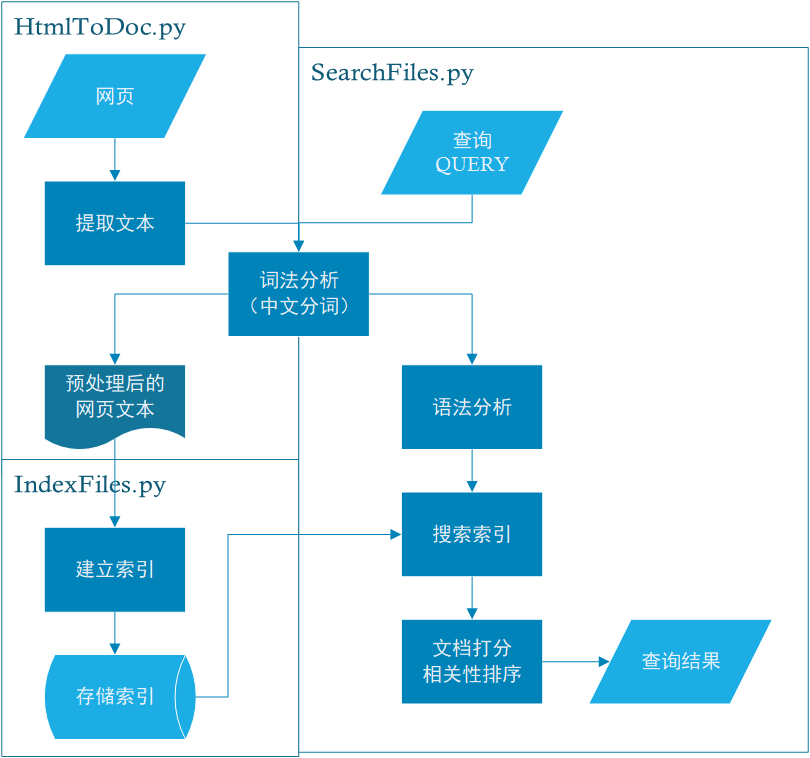
\includegraphics[width=12.5cm]{img/flowchart.png}
\caption{中文网页的建立索引与搜索过程}
\label{fig:flowchart}
\end{figure}

如图\ref{fig:flowchart}所示,本实验的实现分为3个部分。首先,针对中文网页的特点,我们需要对已爬取的中文网页进行解析,利用BeautifulSoup库提取出网页中的文本信息,随后,我们利用现有的中文分词库将中文文本信息进行分词,经过分词后的网页会以文本文档的形式存储下来。在第二部分,我们为这些文档建立索引,建立索引的过程用到了lucene库,可以通过修改样例代码实现。最后,对用户输入的查询语句,我们用同样的中文分词库进行分词,利用lucene库的样例代码从已建立的索引中进行检索、打分、排名,实现中文网页的索引和搜索。


\section{实验步骤}
\subsection{索引的建立}


\subsubsection{Solution}

实验所给的样例代码中,已给出了英文文本的分词和建立索引的实现。在本部分中,我们需要从网页中提取文本内容,并对中文文本进行分词,根据实验的要求建立合适的索引。

\paragraph{提取文本内容}
BeautifulSoup中内置了一个get\_text()函数,能够提取出被解析网页中的所有文本。但get\_text函数还会将javascipt、CSS代码等内容一并返回,针对这一问题,我们在调用get\_text函数之前,先利用BeautifulSoup将HTML树中的script、style标签删除(extract)\footnote{参考:https://stackoverflow.com/questions/22799990/beatifulsoup4-get-text-still-has-javascript},随后再对HTML树调用get\_text函数,我们可以得到较为纯净的中文文本。主要代码如下所示。在提取文本内容时,为方便后续建立索引时为索引文档添加页面标题、url等附属信息,我们还将HTML树中的title标签提取出来,输出在文本文档的第一行。

\begin{python}
path = os.path.join(root, filename)
content = open(path)                                # 获取页面HTML文档
soup = BeautifulSoup(content,features='lxml')       # 解析文档
content.close()
output = open(os.path.join(storeDir, filename),'w')
title = soup.title.string
output.write(title+'\n')                            # 在文本文档第一行输出标题
for script in soup.find_all(["script","style"]):
    script.extract()                                # 删除页面中的js、CSS代码      
text = soup.get_text(strip=True)                    # 提取文本,strip=True表明去除空格、换行符
\end{python}

\begin{figure}[htbp]
\centering
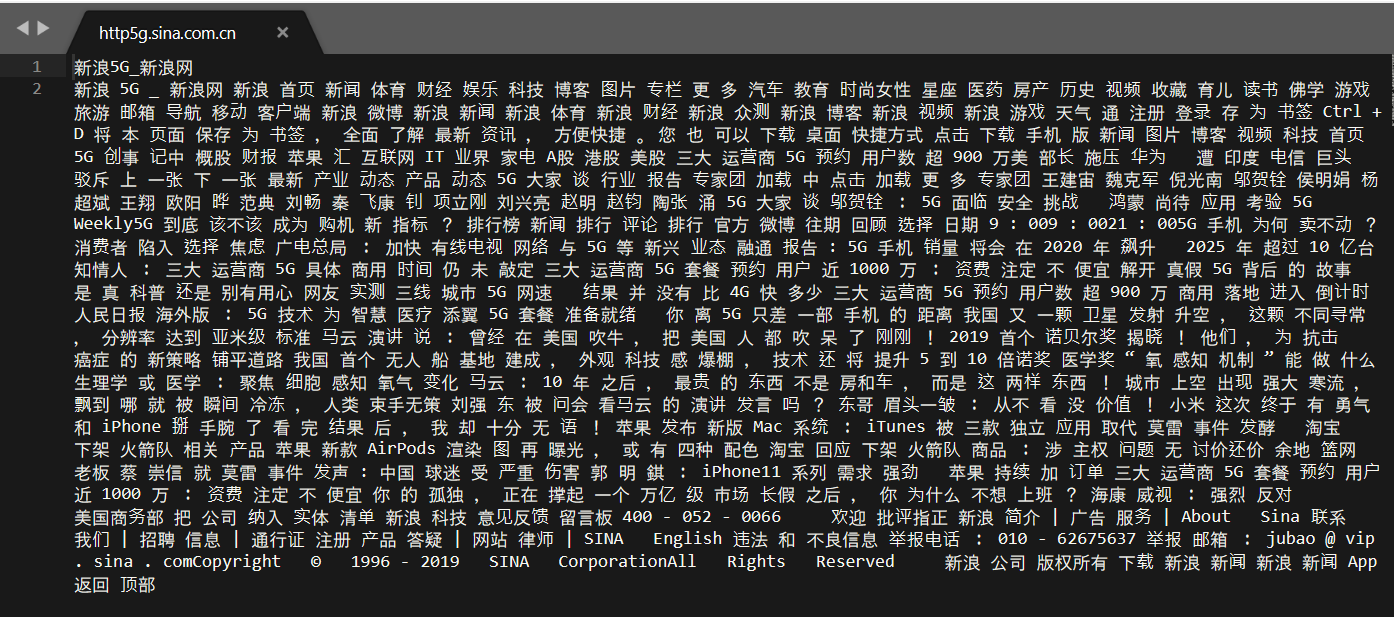
\includegraphics[width=8.5cm]{img/jiebadoc.png}
\caption{中文分词的结果}
\label{fig:jiebadoc}
\end{figure}


\paragraph{中文分词}
在Lucene中,虽然提供了针对中文文本的分词analyzer,但其功能较为单一,仅根据相邻文字进行分词,索引效果较为不理想。为此我们利用了“结巴中文分词器”\footnote{https://github.com/fxsjy/jieba},该分词器能够将连续的中文文本按照词语语义分割成一个连续的词语列表。我们将分词的结果以空格间隔的方式输出到文本文档中。在建立索引的过程中,利用Lucene中的WhiteSpaceAnalyzer,索引器能够直接利用中文分词的结果建立倒排索引,并按我们的需求统计中文单词的词频和位置。在HtmltoDoc.py中,中文分词的相关代码如下所示。中文分词的结果示例如图\ref{fig:jiebadoc}所示。

\begin{python}
def HtmlToDoc(root,storeDir):
    if not os.path.exists(storeDir):
        os.mkdir(storeDir)
    for root, dirnames, filenames in os.walk(root):
        for filename in filenames:
            try:
                output = open(os.path.join(storeDir, filename),'w')
                ...
                seg_list = jieba.cut(text)          # 中文分词
                output.write(" ".join(seg_list))    # 将分词结果以空格间隔输出
                output.close()
            except Exception, e:
                print "Failed in indexDocs:", e

HtmlToDoc("html","docs")
\end{python}


\paragraph{索引的配置}
针对中文空格分词的特点,在本阶段我们采用的分词器是WhiteSpaceAnalyzer,它会读取我们通过空格分割的中文词语,并对文档内容建立倒排索引表。根据题目要求,我们在本阶段建立的索引需要包含有name(文件名),path(文件路径),title(网页标题),url(网页地址)和contents(索引的文件内容)等信息。在索引中,这些特定类型的相关信息被称为域(field)。针对不同信息种类的特点,本实验中我们配置了如下几类域。
\begin{table}[h]
\begin{center}
\begin{tabular}{cccccc}
\hline
\textbf{Field Type} & \textbf{Field Name} & \textbf{Indexed} & \textbf{Stored} & \textbf{Tokenized} & \textbf{\begin{tabular}[c]{@{}c@{}}Record Freq\\ \& Position\end{tabular}} \\ \hline
\textbf{t1}         & path, url, name     & N                & Y               & N                  & N                                \\
\textbf{t2}         & contents            & Y                & N               & Y                  & Y                                \\
\textbf{t3}         & titles              & Y                & Y               & Y                  & Y                                \\ \hline
\end{tabular}
\end{center}
\end{table}

其中文件路径、文件名、URL是文档的固有属性,因此只需要存储而不需要被索引,文档的文本内容是一定会被检索的部分,因此我们建立了分词索引,并统计了词频和位置,考虑到文档内容较为繁多,在本实验的索引建立中,我们暂时不考虑存储文档内容的需求。文档的标题作为文档的固有属性需要被存储,虽然在本实验中不要求被检索,但考虑到标题也包含了重要的文档信息,因此也在这里被分词、统计,加入了索引以备不时之需。


\paragraph{为索引添加文档}
在配置完索引的fieldType后,我们为每一个网页建立相应的索引文档,其中文档路径(path)、文档名称(name)可以不难通过Python中的os库得到,文档的标题(title)、待检索内容(contents)能够直接从与文件名对应的中文文本文档中得到。但网页文档中并没有包含我们所需要的URL信息。这里我们会用到此前爬虫脚本所生成的文档目录index.txt文件,其中记录了每个爬取过网页的文件名和对应的URL信息。为方便起见,我们此处的遍历对象不再是此前的文件目录(os.walk(root)),而是index.txt记录文件的每一行。根据index.txt每一行的第一项,我们可以得到一个URL,再在文档目录中,寻找与第二项文件名所匹配的中文分词文档,将其中的对应信息加入索引文档的对应域中。通过这种方式,我们就可以完成一个网页索引的建立。indexFiles的主要代码如下。

\begin{python}
while True:
    t = indextxt.readline()
    if (len(t) == 0):
        indextxt.close()
        return
    t = t.split()
    filename = t[1]                           # 获取文件名
    URL = t[0]                                # 获取URL
    print "adding", filename
    try:
        path = os.path.join(root, filename)   # 获取文件路径
        file = open(path)
        title = file.readline()               # 打开中文分词处理后的文件,读取第一行的标题
        contents = unicode(file.read())       # 将剩余的内容全部读取
        file.close()
        doc = Document()
        doc.add(Field("name", filename, t1))  # 添加文件名等信息
        ......
        writer.addDocument(doc)
    except Exception, e:                      # 异常处理
        print "Failed in indexDocs:", e
\end{python}


\subsubsection{Results}
运行以上的脚本,我们可以为中文网页建立检索的索引,执行过程截图如图\ref{fig:indextext}所示。


\begin{figure}[hbp]
\centering
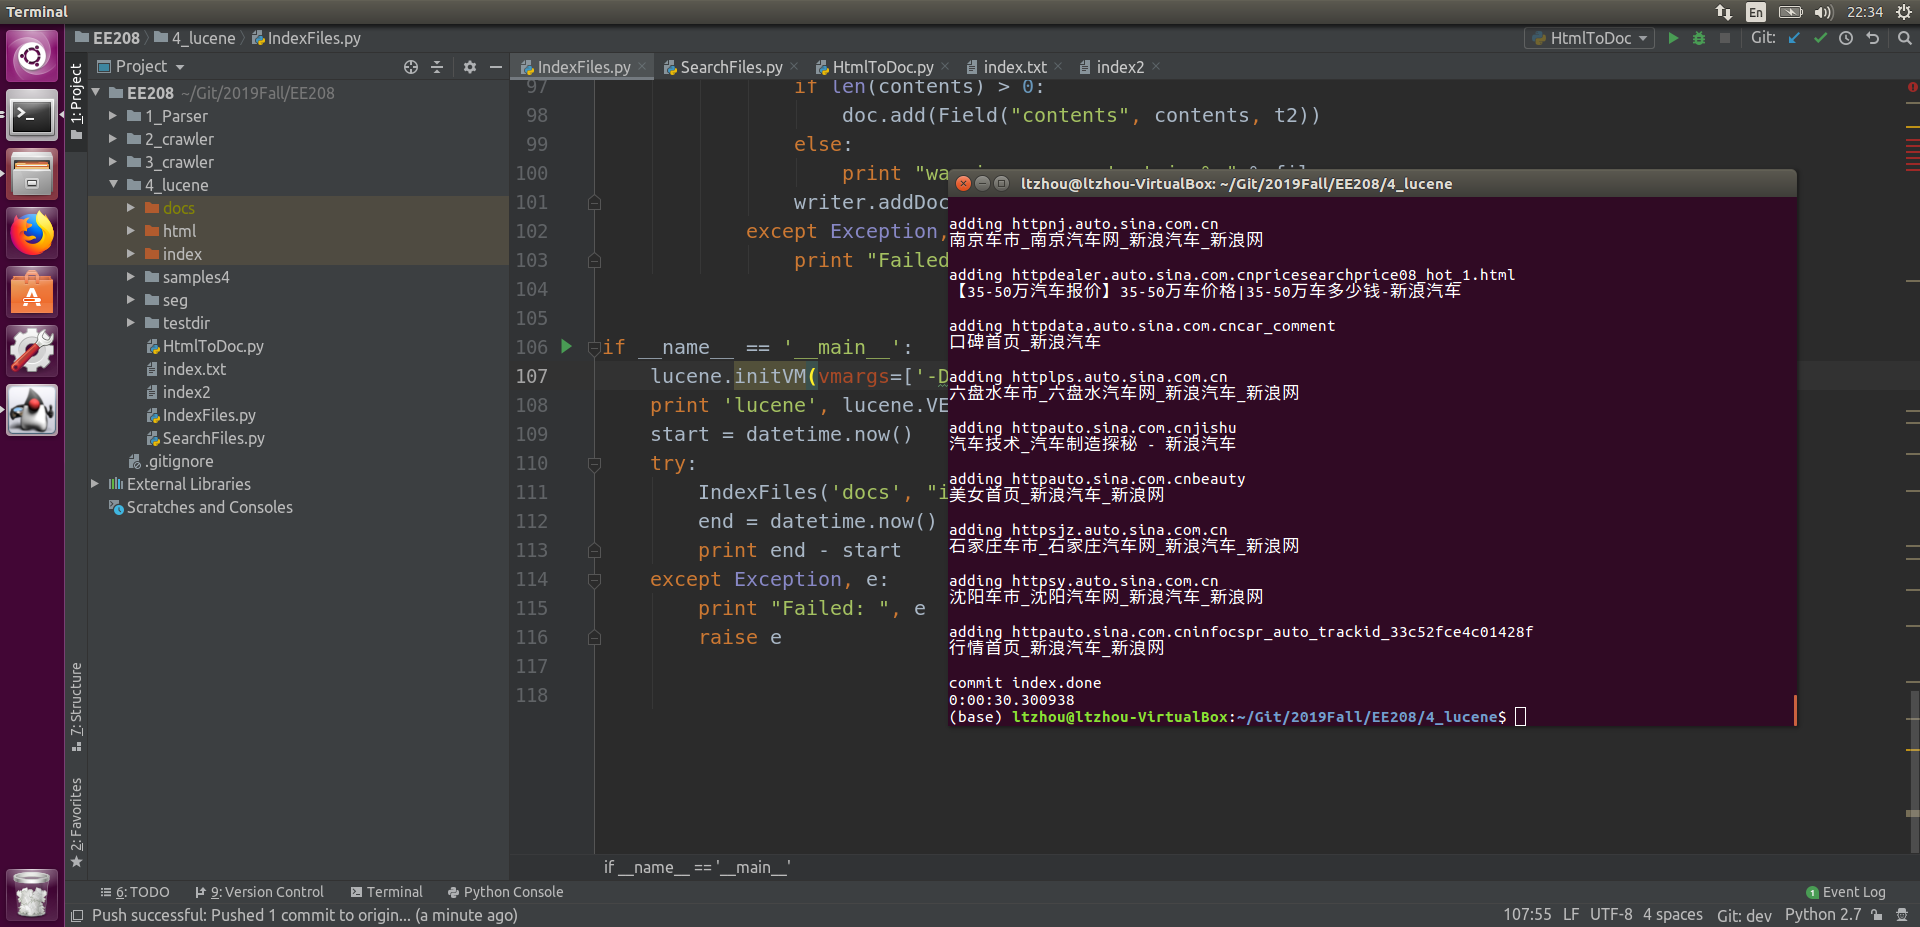
\includegraphics[width=14.5cm]{img/indextext.png}
\caption{建立索引的过程}
\label{fig:indextext}
\end{figure}


\subsection{搜索程序}
\subsubsection{Solution}
\paragraph{分析查询请求}
分析用户输入的查询请求要求我们使用和检索一样的分词器,因此在检索程序的构造中,我们也调用了结巴中文分词库和空格分词器WhiteSpaceAnalyzer。代码如下所示。

\begin{python}
def run(searcher, analyzer):
    while True:
        print
        print "Hit enter with no input to quit."
        command = raw_input("Query:")
        command = unicode(command)
        seg_list = jieba.cut(command)
        command = (" ".join(seg_list))
        if command == '':
            return
        ... # call query parser using WhitespaceAnalyzer
if __name__ == '__main__':
    ...
    analyzer = WhitespaceAnalyzer(Version.LUCENE_CURRENT)
    ...
    run(searcher, analyzer)
    
\end{python}

接下来我们可以将经过解析的Query语句(经过中文空格分词,支持布尔查询)传入检索器searcher,在此前创建的索引中检索信息,打分排序并依次输出。这一部分的代码与示例代码相同。将检索得到的匹配文档中URL、标题等信息输出,我们就完成了搜索程序的构造。

\subsubsection{Results}
实验结果截图\ref{fig:test1},\ref{fig:test2},\ref{fig:test3} 所示。以下的截图中,图\ref{fig:test1}和\ref{fig:test2}展示了一般的关键词搜索结果。图\ref{fig:test2}和\ref{fig:test3}的对比则表明检索器实现了排除NOT命令后的关键词,支持布尔查询。

\begin{figure}[htbp]
\centering
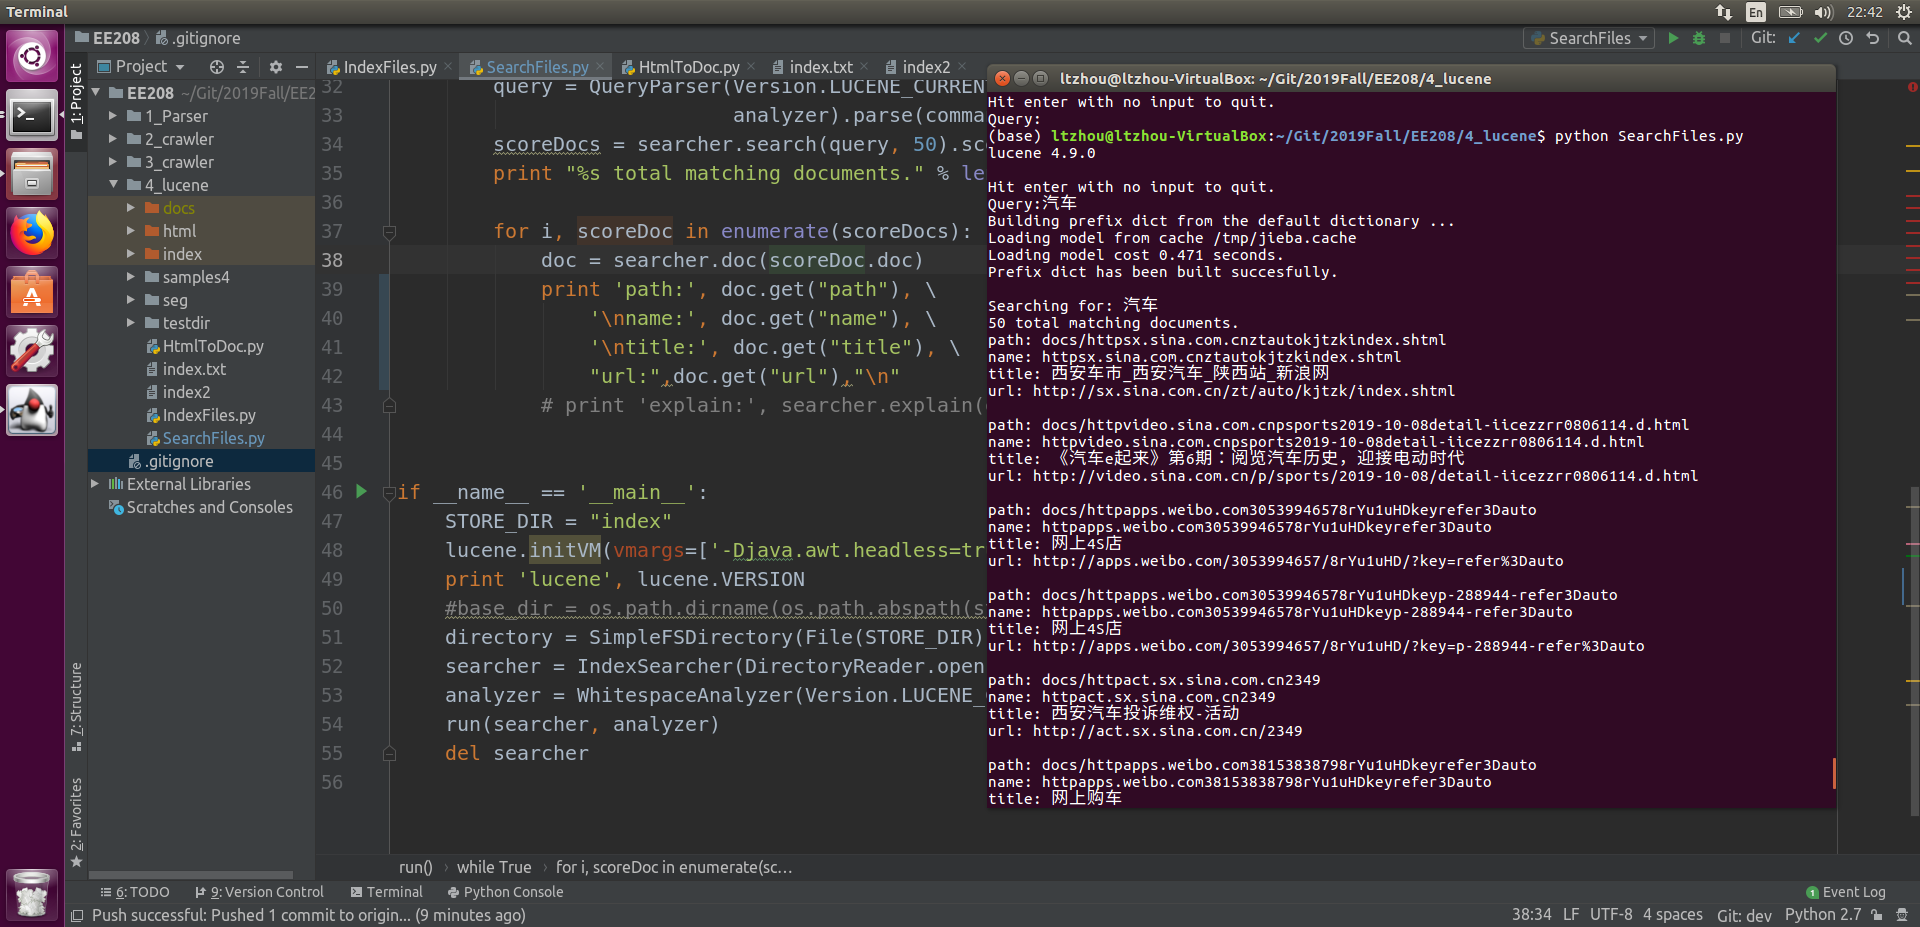
\includegraphics[width=14.5cm]{img/test1.png}
\caption{“汽车”关键词的搜索结果}
\label{fig:test1}
\end{figure}

\begin{figure}[htbp]
\centering
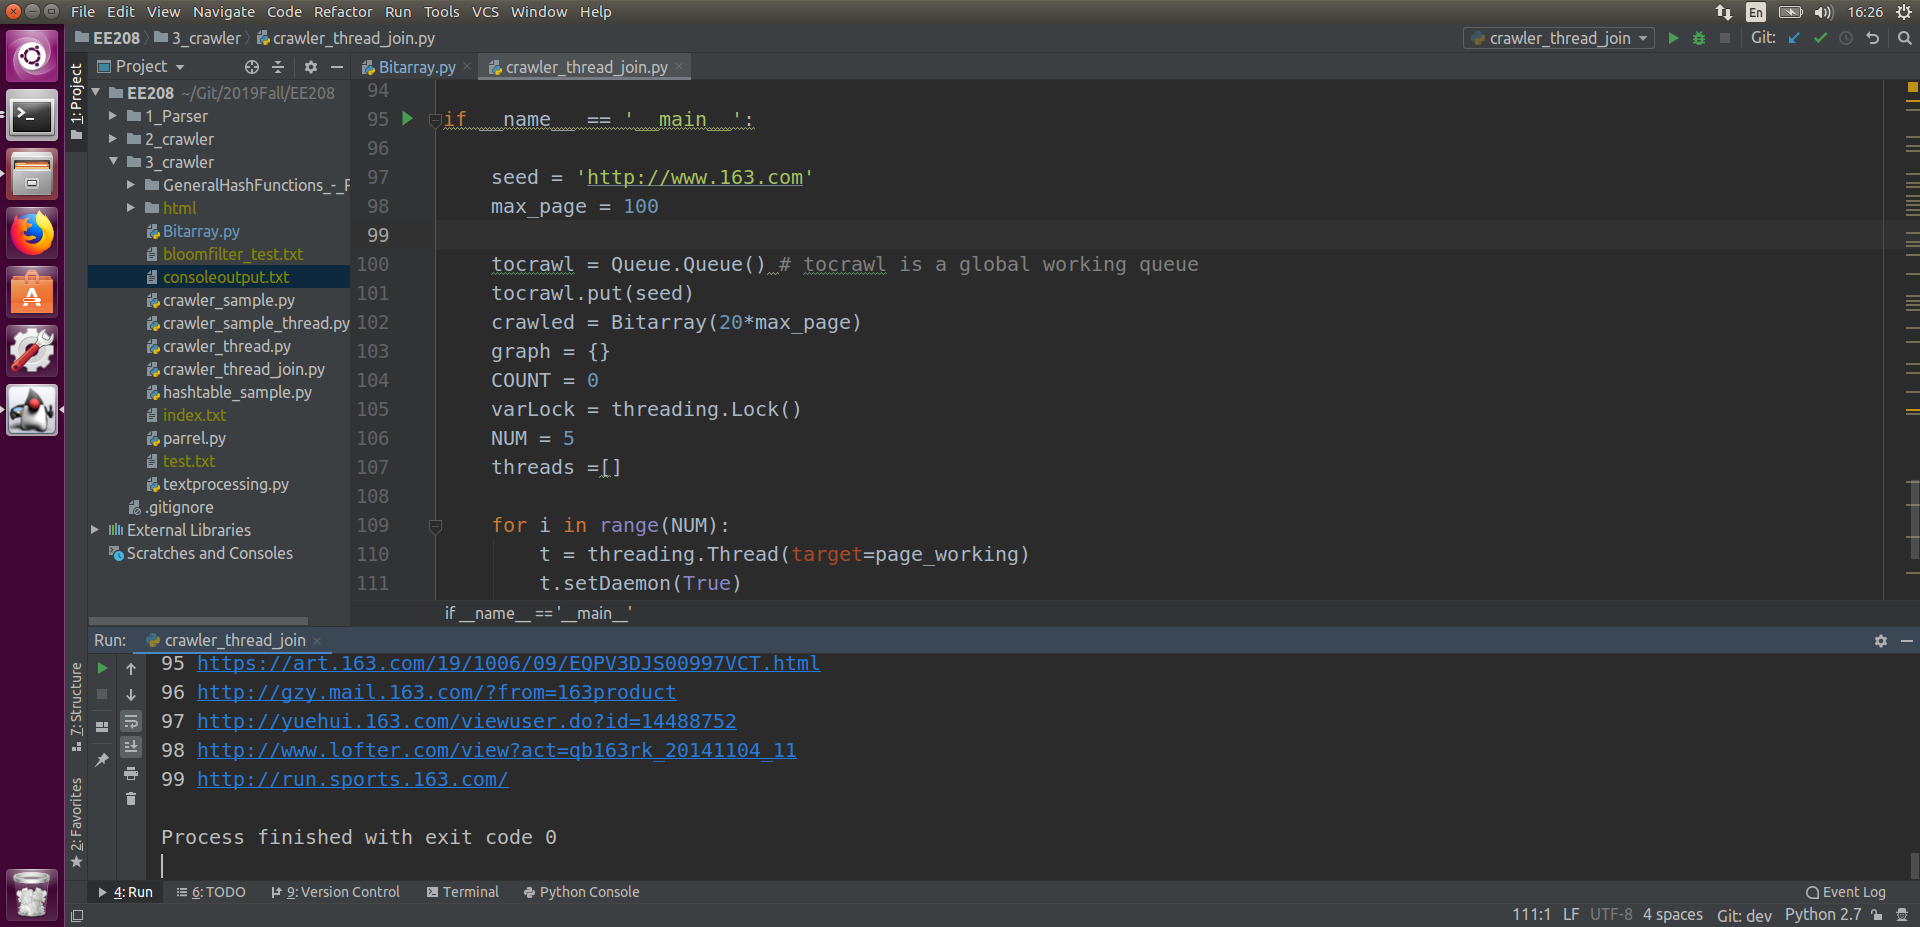
\includegraphics[width=7.5cm]{img/test2.png}
\caption{“上海”关键词的搜索结果}
\label{fig:test2}
\end{figure}

\begin{figure}[htbp]
\centering
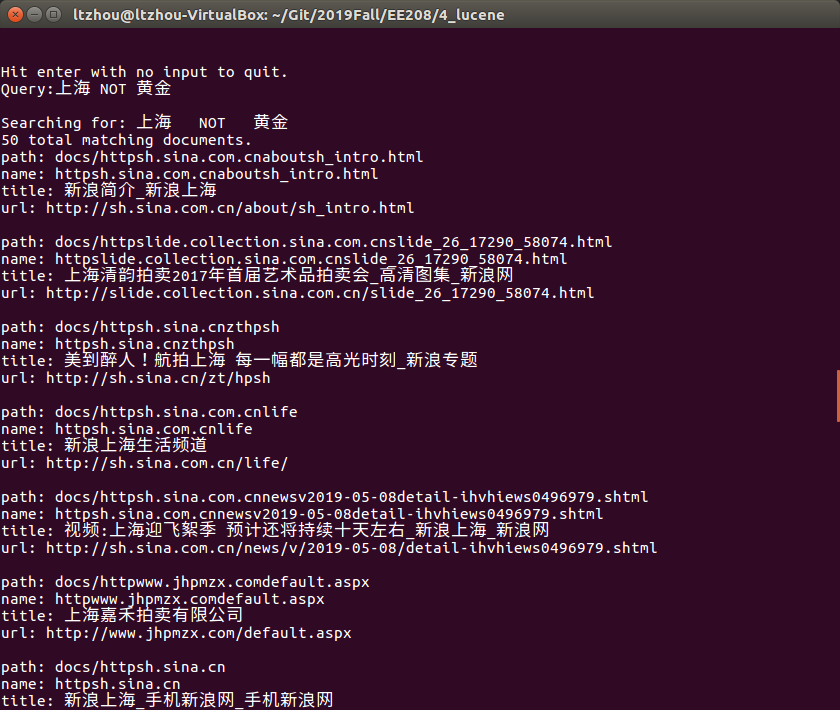
\includegraphics[width=7.5cm]{img/test3.png}
\caption{排除“黄金”后,“上海”关键词的搜索结果}
\label{fig:test3}
\end{figure}


\section{实验总结}
\paragraph{概述}
通过本次实验的学习,我将课堂上学习到的建立索引表、词法分析、文档打分等概念付诸实践,学会了如何利用lucene搭建一个简单的搜索引擎。

\paragraph{感想}
为了提高搜索引擎的检索效果,构建索引的过程十分重要,我们的索引应该能够完备、有效地描述一个网页中主要的文字内容。在最初,我使用了一个简单的get\_text函数提取网页上的文本,这样做所带来的问题是我们所提取出的文字中,大量javascript、CSS代码被识别成文本保留了下来,对这些代码做索引是没有意义的,这将降低搜索引擎的表现。在通过网络获得帮助,对提取文本的函数经过改进后,我们的中文搜索引擎能够达到良好的检索效果。这带给我的启示是在对网页建立索引时,我们需要灵活根据需要提取有用的信息,避免冗余信息影响索引的构建和检索的效果。

\paragraph{创新}
在本实验中,我新建了一个将中文网页提取文本、进行分词的函数(HtmltoDoc.py)。该函数能够将一个目录下的HTML文件进行解析,提取出其中的文本,并利用结巴分词器进行分词,将分词结果输出在另一个目录下的同名文件中。该函数能够独立地被调用,用于网页信息的预处理、检索索引的建立等场合中。


\paragraph{问题}
本实验中遇到的主要问题是提取文本时,BeautifulSoup库会保留大量代码。参考网络上的信息,我设计了一个操作,先将HTML树中包含大量代码的style、scipt标签剔除,再调用get\_text函数,实现了文本的有效输出,解决了这一问题。

\end{document}

